\begin{bibunit}[IEEEtran.bst]

  \chapter*{Modeling and solving altimetry problems}
\addcontentsline{toc}{chapter}{Modeling and solving altimetry problems}
  \chaptermark{Modeling and solving altimetry problems}
  
\begin{figure}[h]
    \centering
    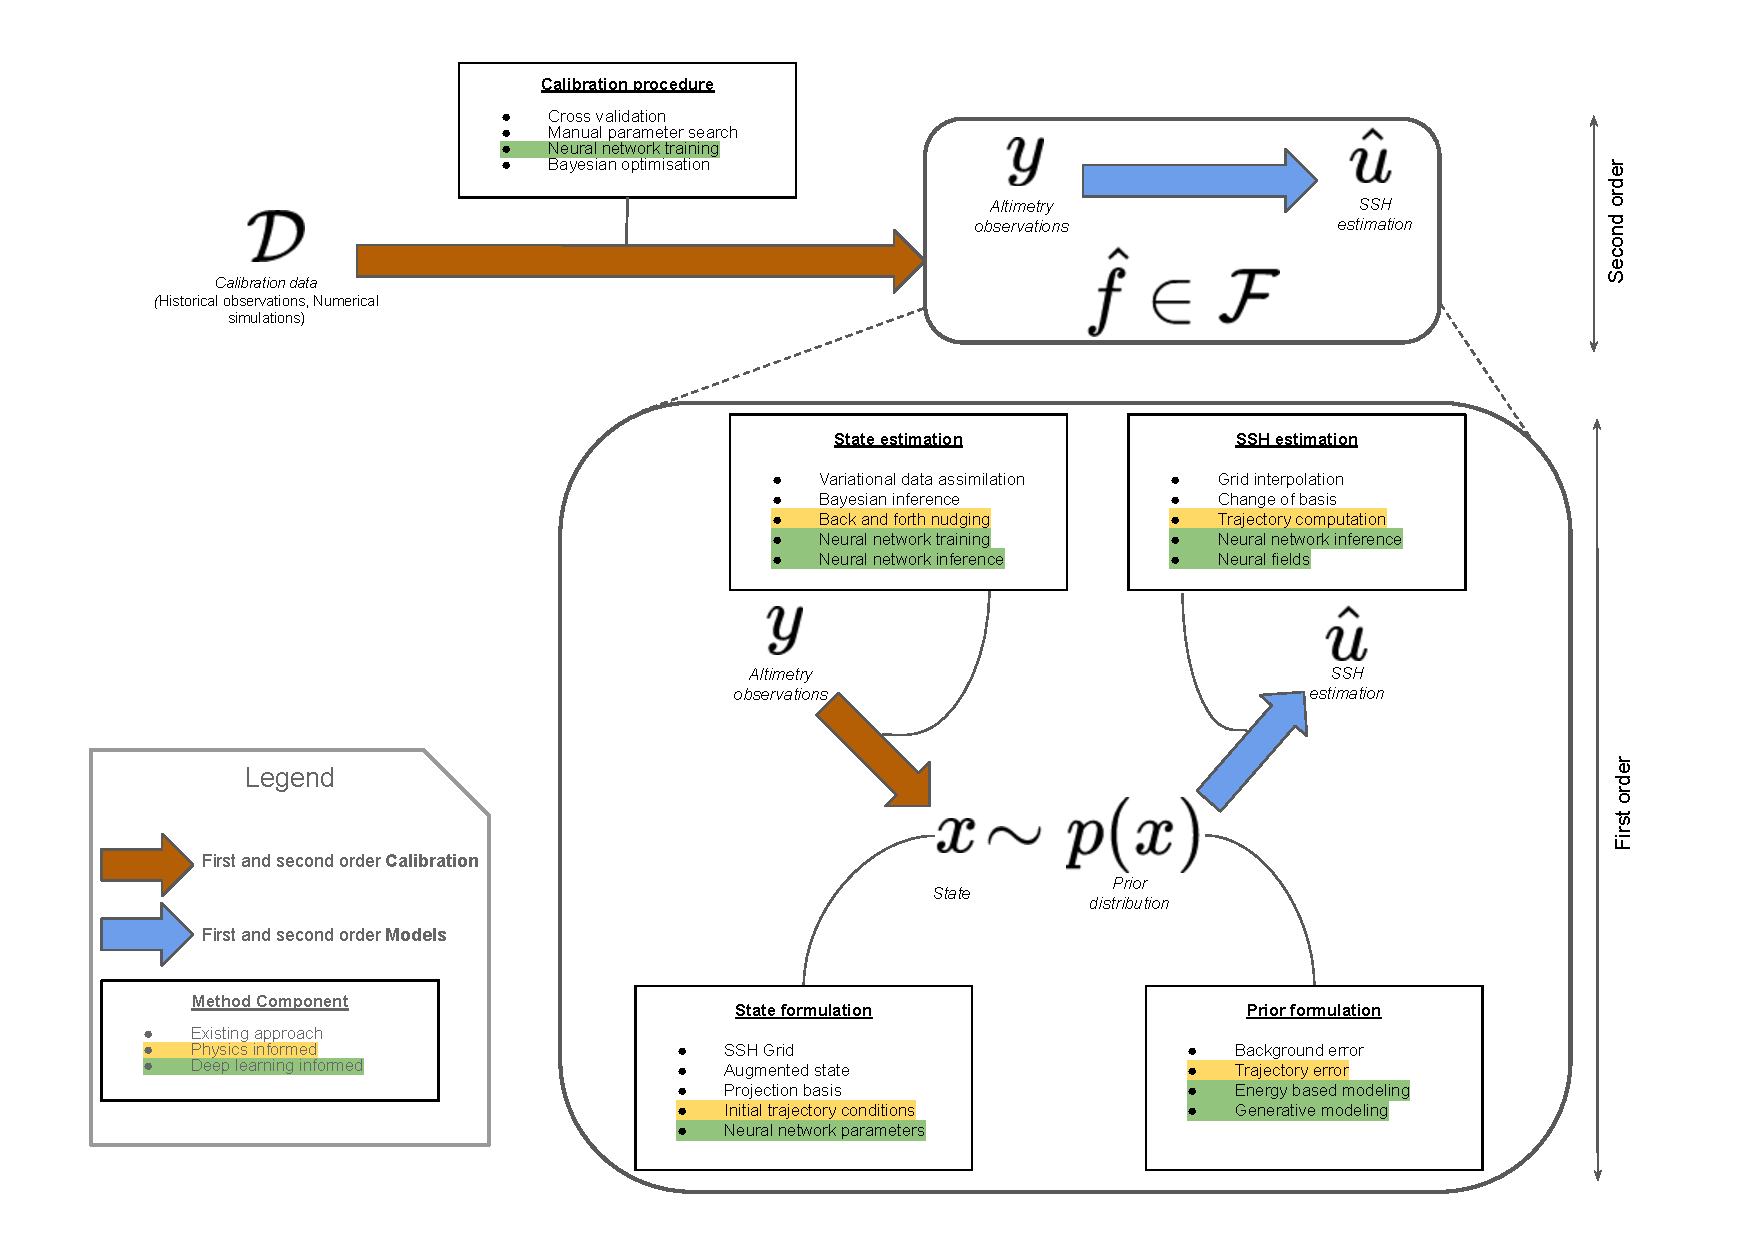
\includegraphics[width=\textwidth]{00_LitReview/Methodology.pdf}
    \caption{\textbf{Solving altimetry problems}. This figure displays the different methodological components in play when addressing an altimetry challenge. The different approaches for each component are detailed and we highlight which ones are physics or deep learning inspired. The specific methods using are detailed below}
    \label{fig:method}
\end{figure}

This chapter uses the methodological framework presented in the introduction to discuss various existing methodologies for modeling and addressing issues related to ocean altimetry. The final section delves into the specifics of the 4DVarNet framework, which serves as the backbone for the research presented in this thesis.



Our attention is primarily directed towards techniques that are pertinent to the altimetry challenges explored in this study. Most existing methods are geared towards altimetry mapping, as calibration of the Surface Water and Ocean Topography (SWOT) mission is a relatively nascent area with fewer established techniques. Nonetheless, both types of problems aim to estimate the sea surface height $u$ given observations $y$.



 
 \section{Priors: Assumptions on Sea Surface Height (SSH)}
The first distinguishing feature among various methods is the assumptions made about the SSH field $u$. These assumptions can be categorized into two types.
The first type involves the choice of representation $x$ for the target SSH field $u$. This representation essentially outlines the space of all possible SSH states.
The second type of assumption aims to characterize the probability distribution $p(x)$ of $x$, describing which states are more likely a priori.



 
  \subsection{State representation}
Choosing a state representation is equivalent to determining the quantities that characterizes the state and the relationship between the state values $x$ and the estimated SSH field $\hat{u}$.


  Looking at existing methods, the SSH field can be characterized through values sampled on a grid or mesh of the domain. These values can directly represent SSH as represented by methods such as the DUACS optimal interpolation \cite{taburetDUACSDT2018252019} (OI), quasi-geostrophic back and forth nudging (BFN-QG) \cite{guillouMappingAltimetryForthcoming2021}, Kalman filtering in GLORYS12 reanalysis \cite{lelloucheCopernicusGlobal122021} or Dynamical Interpolation \cite{ubelmannDynamicInterpolationSea2015,ballarottaDynamicMappingAlongTrack2020} .
  Other methods chose more complex description of the SSH values with large scale and small scale components like in the 4DVarNet\cite{beauchamp4DVarNetSSHEndtoendLearning2023} or even projected values on another basis like MIOST\cite{ubelmannReconstructingOceanSurface2021,ubelmannSimultaneousEstimationOcean2022} which uses a wavelet basis.
  The choices like the mesh, basis or SSH decomposition used is a way to use prior knowledge to dimension the state space. A grid representations of the SSH can be propagated to the whole domain $\Omega_u$ using interpolation schemes which impose additional choices.

  The strongly constrained four dimensional variational data assimilation (s4DVAR)\cite{carrassiDataAssimilationGeosciences2018} characterizes the SSH field over a period through the initial conditions. A dynamical model $\mathcal{M}$ and an associated numerical forecast scheme  is then used to infer the SSH over the whole temporal horizon. Note that the initial condition is usually also represented on a grid and implies similar choices as before. 

Deep learning has introduced new ways of representing the SSH. Notably, Neural fields\cite{johnsonNeuralFieldsFast2022} consists in describing the SSH with the parameters of a coordinate-based neural network $\eta$. The neural network can then be used to output the SSH value for any given coordinate of the domain.


Finally the state can also contain ancillary quantities that are linked to the SSH. In the GLORYS12\cite{lelloucheCopernicusGlobal122021} reanalysis, the data assimilation scheme considers the state of the ocean beyond the SSH. 
In the case of the SWOT calibration, estimating the SSH is equivalent to estimating the error signals. Operational methods\cite{dibarboureDataDrivenCalibrationAlgorithm2022} approach the problem as defining a state representation of the different error signals making assumptions on the processes generating them.

\subsection{Prior on the state space}
The representation of SSH $x$ we chose defined the space of all possible states. Additional assumptions can be made to specify which states are more likely than others. This is the prior distribution of the states $p(x)$.
Some approaches like existing work Neural fields do not define an explicit prior distribution over the state space, which implies a uniform distribution.
Other like OI and s4DVAR shape $p(x)$ through a background state $x_b$ and an error covariance matrix $B$. Under Gaussian assumptions, the prior distribution becomes 
 $$\mathcal{p}(\mathbf{x}) = \frac{1}{\sqrt{(2\pi)^n |\mathbf{B}|}} \exp\left(-\frac{1}{2} (\mathbf{x} - x_b)^T \mathbf{B}^{-1} (\mathbf{x} - x_b)\right)$$

In Kalman filters, 3DVAR or weakly constrained four dimensional variational data assimilation (w4DVAR), the likelihood of a state is based on its distance to the trajectory of a dynamical model rather than to a background state giving a similar formulation as above but with $x_b$ replaced by a state-dependent quantity.

Deep learning also introduces tools for probabilistic and energy-based modeling that can be used to characterize $p(x)$.
 For example, 4DVarNet employs a neural network $\phi$ to define the following quantity over the state space $\| x - \phi(x)\|$. Interpreting this as an energy function, a Boltzmann distribution over $\chi_x$ can be defined, yielding the prior distribution
 $$p(\mathbf{x}) = \frac{\exp(-E(\mathbf{x}) / T)}{Z}$$
 with $Z = \int \exp(-E(\mathbf{x}) / T) \, d\mathbf{x}$ and $T$ the temperature parameter.



We summarize in the table below the different approaches.
  \begin{table}
  \centering
\begin{tabular}{|l|l|l|l|}
\hline
  Method & State formulation & SSH estimation &  Prior formulation\\
\hline
  OI & SSH Grid & Grid Interpolation & Background error \\

  KF, 3DVAR $^{(*)}$ & SSH Grid at time $t$ & Grid Interpolation & Trajectory error \\

  s4DVar & Initial conditions & Trajectory computation & Initial background error \\

  w4DVar & SSH Grid & Grid Interpolation & Trajectory error \\

  MIOST & Wavelet components & Basis change  & Background error \\

  4DVarNet & Scale components & Sum + Grid estimation  & Energy-based model \\

  Neural field & NN parameters & NN inference & None (Uniform) \\
\hline
\end{tabular}
\caption{\textbf{Comparison of SSH models across various methods}. The columns indicate the type of state representation $x$, the method of obtaining estimated SSH $\hat{u}$, and the prior distribution $p(x)$.}
\end{table}



\section{Solvers: Estimating the state given some observations}

Once all prior assumptions about the SSH field have been made (i.e. the first order \textbf{model}), the methods differ by the choice of \textbf{calibration procedure} $\gamma$. $\gamma$ defines how to estimate the state $\hat{x}$ given some observations $y$ defined on a domain $\Omega_y$.

This problem can be framed as an inverse problem by defining an observation operator $H$ that describe the relation from state to observations ($\gamma$ then becomes the inverse $H$).
We define the estimated observations as $\hat{y} = H(x)$. For altimetry observations that measure the quantity of interest $u$, the $H$ operator can be decomposed as $H(x) = \hat{u}_x(\Omega_y) + \epsilon$ with $\epsilon$ an error term and $\hat{u}$ the estimated SSH for a given state $x$ as introduced in the previous section. The field of data assimilation in geoscience propose a variety of methods to solve inverse problems.

Using a Bayesian inference formulation, the estimate of the posterior state is done by assuming Gaussian distributions for observation errors and prior states. 
For Optimal Interpolation, this can be mathematically expressed as:
 $$\gamma(y)= x_b + K(y - Hx_b)$$
with $K$ is the Kalman gain and $H$ is a linear observation operator and $x_b$ the background state.
Kalman filters use a similar expression which is applied sequentially for each time step.
The procedure $\gamma$ then becomes a sequence of sub-procedure $\gamma_{t1}, ..., \gamma_{t_n}$ applied to observations $y_{t1}, ..., y_{t_n}$ to estimate the states $x_{t1}, ..., x_{t_n}$ 
$$\gamma_{t+1}(y_{t+1})= x_{t} + K_{t+1}(y_{t+1} - H_{t+1}M_{t:t+1}x_{t})$$
 with $M_{t:t+1}$ a linear forecast operator.


Variational methods solve the estimation as an optimization problem. The objective is framed as the minimization of a variational cost $\gamma(y) = \arg\min_x J(x, y)$ that includes a observation term $J_{obs}(x, y)$ and a regularization term  $J_{reg}(x)$ related to the prior distribution. The formulation is:

$$ \gamma(y) = \arg\min_x \left[ J_{\text{reg}}(x) + J_{\text{obs}}(x, y) \right]$$
The minimization procedure is classically performed using an iterative gradient based algorithm\cite{carrassiDataAssimilationGeosciences2018}. The gradients can be computed using the adjoint method\cite{lelloucheCopernicusGlobal122021} or automatic differentiation libraries in deep learning\cite{fablet_end2end_2021}.
The calibration of neural fields is also framed as a the minimization of a training objective. However in existing work \cite{johnsonNeuralFieldsFast2022}, since no prior distribution is defined over the states, the variational cost effectively contains only on the observation term.
Such methods are used in variational data assimilation such as 3DVAR, strong and weak 4DVAR, 4DVarNet and can be used to solve the OI problem. Note that similarly to Kalman filters, the 3DVAR method also perform a sequential resolution of the estimation.


Deep learning offers alternative strategies such as direct inversion, where a neural network directly models the function $\gamma$. This eliminates the need for explicitly defining an inverse problem and prior distribution. Example of this approach using classical computer vision models have been applied to altimetry mapping in \cite{manucharyanDeepLearningApproach2021a} and we apply this method in Chapter 3 for SWOT calibration applications.


The different calibration procedures of different methods are summarized in the table below 

\begin{table}
  \centering
  \begin{tabular}{|c|c|c|}
\hline
    Methods & Procedure $f$ \\
\hline
    3DVAR$^{(*)}$, w4DVAR, OI, 4DVarNet & Variational data assimilation \\
    OI, Kalman filters$^{(*)}$ & Bayesian inference \\
    Direct inversion, 4dVarNet & NN inference \\
    Neural fields & Neural network training \\
\hline
\end{tabular}
\caption{\textbf{Comparison of state estimation strategies for existing altimetry methods} $^{(*)}$ indicate the method that use a sequential resolution.}
\end{table}

% | Methods    |         estimation         |   O(y, x)   |
% | ---------- |:--------------------------:|:------------:|
% | Nerf       | $\theta = argmin(\cal{L})$ |  $\cal{L}$   |
% | Var        |      $ x = argmin(\alpha R(z) + \beta O(y, x))$      |    $\|y - Hx\|$          |
% | OI, Kalman | $x = x_b + K(y - Hx_b)$ | $\|y - Hx\|$ |
% | Direct Inv |          $x = \phi(y)$          |              |
%




\section{Calibrating the method}
The choice of prior formulation and estimation procedure provide a method with free parameters (i.e. second order \textbf{model}) that need to be calibrated. 
Calibrating the method involves the fine-tuning of several parameters and model factors. These include the background field, covariance matrices for observation and background errors, as well as specifics for variational optimization or numerical model integration. In the case of deep learning approaches like direct inversion, the parameters of the neural network also become factors requiring calibration.


The calibration process relies on datasets, typically comprising numerical model outputs and pre-existing observations. These data sets serve for estimating the aforementioned factors and for validating the performance of the state estimation procedure.
A widely adopted approach for this calibration is cross-validation. In this technique, a subset of available data is utilized to configure the model, which is then tested on the remaining data to evaluate its performance. The exploration of possible configurations may range from manual adjustments to automated parameter tuning algorithms, depending on the complexity of the method being calibrated.

For methods incorporating neural architectures, advanced optimization algorithms specific to deep learning are often employed. These algorithms efficiently tune the weights and biases of the neural network, aligning them for better performance in the SSH estimation task. This is particularly advantageous for direct inversion approaches, which depend entirely on the data for calibration and do not require explicit prior models.


\section{A closer look on the 4dVarNet}Dans 3 jour il y a
\begin{figure}[h]
    \centering
    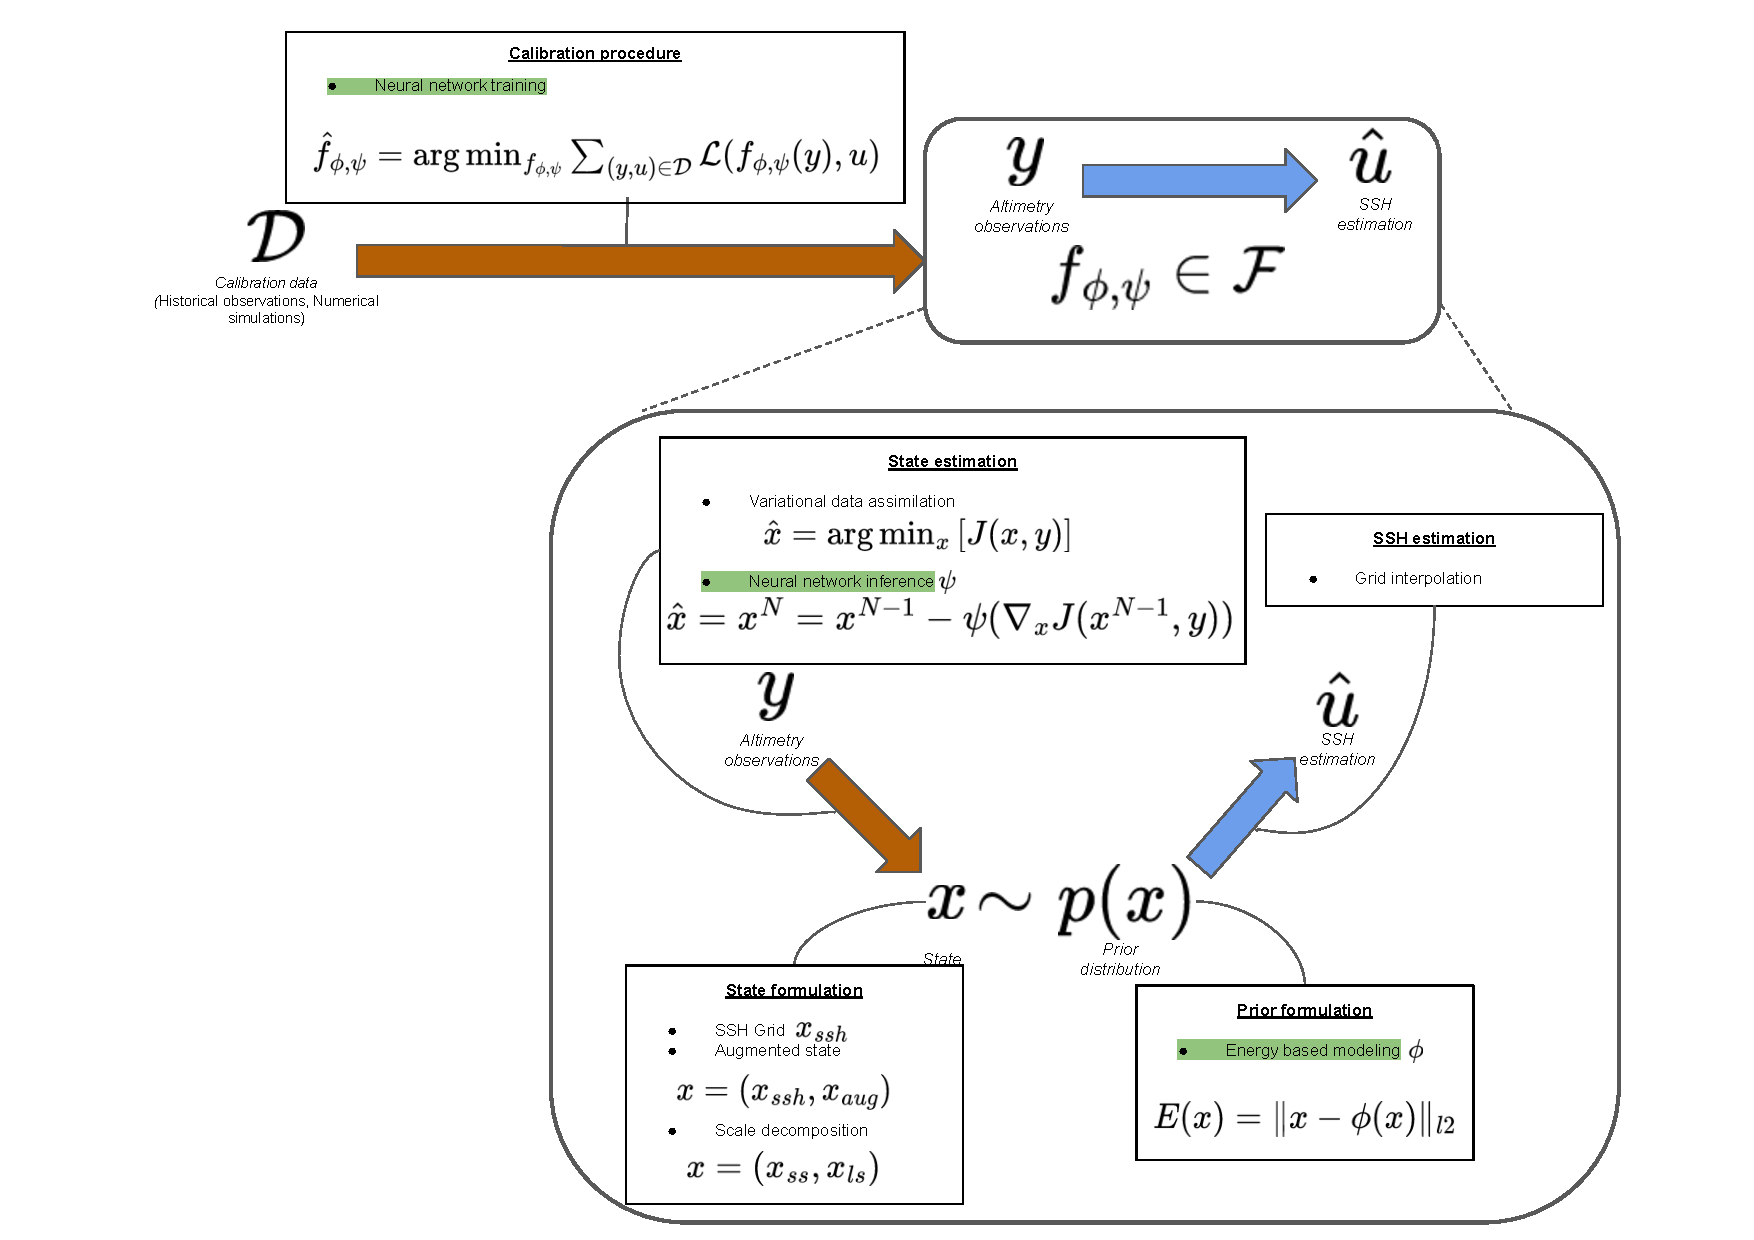
\includegraphics[width=\textwidth]{00_LitReview/Method-4dvarnet.pdf}
    \caption{\textbf{4dVarNet Method}}
    \label{fig:method}
\end{figure}
In this section, we delve into the architecture of 4DVarNet, a prominent framework frequently employed throughout this thesis. 
Introduced as a promising approach for mapping altimetry data, 4DVarNet demonstrated robust performance in a study involving simulated SSH based on NATL60 simulation data\cite{fablet_end2end_2021}. Various regions \cite{beauchamp4DVarNetSSHEndtoendLearning2023} and altimetry configurations were considered in these studies, including setups with 4 nadir altimeters both with and without SWOT observations. Earlier versions considered OI-based products as additional observational data for the inversion \cite{fablet_end2end_2021}.

The representation of the SSH field within the 4DVarNet framework has evolved over time. While earlier studies decomposed SSH into large and small-scale components \cite{beauchampDatadrivenLearningbasedInterpolations2021}, recent implementations used in Chapter 4 represent directly the SSH grid points a single scalar values. In  \cite{fablet_end2end_2021}, latent variables are added to the state to enrich the prior distribution over the state space without being directly constrained by the observations.

The framework employs a neural network, denoted as  $\phi$  or the formulation of the prior cost as $J_{reg}= \|x - \phi(x)\|_{l2}$ using an $l2$ norm.
Most altimetry studies using the 4dVarNet formulate $\phi$ as a multiscale bilinear blocks \cite{fabletBilinearResidualNeural2018}, A simpler single scale is used in Chapter 4. Outside of altimetry, other $\phi$ have been experimented on Lorenz systems including true dynamics\cite{fabletLearningVariationalData2021}

A Gaussian assumption for the observation errors is commonly adopted, articulated through a quadratic norm in the observation cost $J_{obs}= \|y - \hat{u}(\Omega_y)\|_{l2}$. In a study that incorporated Sea Surface Temperature (SST) observations\cite{fabletMultimodal4DVarNetsReconstruction2023}, convolutional filters were used to formulate the observation operator that maps the state to SST.


State estimation in 4DVarNet is tackled as a minimization problem for a variational cost, which is a combination of the observation and regularization costs. The optimization procedure is inspired by meta-learning approaches and employs a Recurrent Neural Network (RNN) to compute state updates at each iteration based on the gradient of the variational cost\cite{fabletENDTOENDPHYSICSINFORMEDREPRESENTATION2021}. Earlier works used fixed-point algorithms for maximizing observation likelihood, followed by a forward pass using the neural network $\phi$ \cite{beauchampDatadrivenLearningbasedInterpolations2021}. 

Apart from the cross validation and exploration of different architectures and configurations, the calibration of the neural network's parameters, both for the solver and the prior, is achieved through the Adam optimization algorithm \cite{kingmaAdamMethodStochastic2017}. The aim is to minimize both the mean squared error in SSH reconstruction and its gradients. To ensure effective weightage in the neural prior, a supplementary term is added to the training loss, constraining the estimated states to have low prior costs.
4DVarNet has emerged as a versatile and effective architecture for handling altimetry data, with various advancements and optimizations over time. By combining neural networks with traditional variational techniques, it opens up promising avenues for state-of-the-art state estimation in oceanographic applications.

\addcontentsline{toc}{section}{Bibliography}
\putbib[./00_LitReview/LitReview-Biblio.bib]
\end{bibunit}

